\documentclass[final]{beamer}\usepackage[]{graphicx}\usepackage[]{color}
%% maxwidth is the original width if it is less than linewidth
%% otherwise use linewidth (to make sure the graphics do not exceed the margin)
\makeatletter
\def\maxwidth{ %
  \ifdim\Gin@nat@width>\linewidth
    \linewidth
  \else
    \Gin@nat@width
  \fi
}
\makeatother

\definecolor{fgcolor}{rgb}{0.345, 0.345, 0.345}
\newcommand{\hlnum}[1]{\textcolor[rgb]{0.686,0.059,0.569}{#1}}%
\newcommand{\hlstr}[1]{\textcolor[rgb]{0.192,0.494,0.8}{#1}}%
\newcommand{\hlcom}[1]{\textcolor[rgb]{0.678,0.584,0.686}{\textit{#1}}}%
\newcommand{\hlopt}[1]{\textcolor[rgb]{0,0,0}{#1}}%
\newcommand{\hlstd}[1]{\textcolor[rgb]{0.345,0.345,0.345}{#1}}%
\newcommand{\hlkwa}[1]{\textcolor[rgb]{0.161,0.373,0.58}{\textbf{#1}}}%
\newcommand{\hlkwb}[1]{\textcolor[rgb]{0.69,0.353,0.396}{#1}}%
\newcommand{\hlkwc}[1]{\textcolor[rgb]{0.333,0.667,0.333}{#1}}%
\newcommand{\hlkwd}[1]{\textcolor[rgb]{0.737,0.353,0.396}{\textbf{#1}}}%
\let\hlipl\hlkwb

\usepackage{framed}
\makeatletter
\newenvironment{kframe}{%
 \def\at@end@of@kframe{}%
 \ifinner\ifhmode%
  \def\at@end@of@kframe{\end{minipage}}%
  \begin{minipage}{\columnwidth}%
 \fi\fi%
 \def\FrameCommand##1{\hskip\@totalleftmargin \hskip-\fboxsep
 \colorbox{shadecolor}{##1}\hskip-\fboxsep
     % There is no \\@totalrightmargin, so:
     \hskip-\linewidth \hskip-\@totalleftmargin \hskip\columnwidth}%
 \MakeFramed {\advance\hsize-\width
   \@totalleftmargin\z@ \linewidth\hsize
   \@setminipage}}%
 {\par\unskip\endMakeFramed%
 \at@end@of@kframe}
\makeatother

\definecolor{shadecolor}{rgb}{.97, .97, .97}
\definecolor{messagecolor}{rgb}{0, 0, 0}
\definecolor{warningcolor}{rgb}{1, 0, 1}
\definecolor{errorcolor}{rgb}{1, 0, 0}
\newenvironment{knitrout}{}{} % an empty environment to be redefined in TeX

\usepackage{alltt}
\usepackage{grffile}
\mode<presentation>{\usetheme{CambridgeUSPOL}}

\usepackage[utf8]{inputenc}
\usepackage{amsfonts}
\usepackage{amsmath}
\usepackage{natbib}
\usepackage{graphicx}
\usepackage{array,booktabs,tabularx}
\usepackage{epstopdf}
\usepackage{colortbl, xcolor}
\newcolumntype{Z}{>{\centering\arraybackslash}X}

% rysunki
\usepackage{tikz}
\usepackage{ifthen}
\usepackage{xxcolor}
\usetikzlibrary{arrows}
\usetikzlibrary[topaths]
\usetikzlibrary{decorations.pathreplacing}
%\usepackage{times}\usefonttheme{professionalfonts}  % times is obsolete
\usefonttheme[onlymath]{serif}
\boldmath
\usepackage[orientation=portrait,size=a0,scale=1.4,debug]{beamerposter}                       % e.g. for DIN-A0 poster
%\usepackage[orientation=portrait,size=a1,scale=1.4,grid,debug]{beamerposter}                  % e.g. for DIN-A1 poster, with optional grid and debug output
%\usepackage[size=custom,width=200,height=120,scale=2,debug]{beamerposter}                     % e.g. for custom size poster
%\usepackage[orientation=portrait,size=a0,scale=1.0,printer=rwth-glossy-uv.df]{beamerposter}   % e.g. for DIN-A0 poster with rwth-glossy-uv printer check
% ...
%

\usecolortheme{seagull}
\useinnertheme{rectangles}
\setbeamercolor{item projected}{bg=darkred}
% \setbeamertemplate{enumerate items}[default]
\setbeamertemplate{caption}{\insertcaption} 
\setbeamertemplate{navigation symbols}{}
\setbeamercovered{transparent}
\setbeamercolor{block title}{fg=darkred}
\setbeamercolor{local structure}{fg=darkred}

\setbeamercolor*{enumerate item}{fg=darkred}
\setbeamercolor*{enumerate subitem}{fg=darkred}
\setbeamercolor*{enumerate subsubitem}{fg=darkred}

\setbeamercolor*{itemize item}{fg=darkred}
\setbeamercolor*{itemize subitem}{fg=darkred}
\setbeamercolor*{itemize subsubitem}{fg=darkred}

\newlength{\columnheight}
\setlength{\columnheight}{100.5cm}
\renewcommand{\thetable}{}
\def\andname{,}
\authornote{}

\renewcommand{\APACrefatitle}[2]{}
\renewcommand{\bibliographytypesize}{\footnotesize} 
\renewcommand{\APACrefYearMonthDay}[3]{%
  {\BBOP}{#1}
  {\BBCP}
}
\IfFileExists{upquote.sty}{\usepackage{upquote}}{}
\begin{document}




\date{}

\author{Piotr Sobczyk\inst{1}, Chris Lauber\inst{2}, Pawe\l{} Mackiewicz\inst{3}, Micha\l{} Burdukiewicz\inst{3}*\\
\normaltext{*michalburdukiewicz@gmail.com} $\diamondsuit$ \normaltext{michbur@github}}

\institute{\small{\textsuperscript{1}Wroc\l{}aw University of Science and Technology, Faculty of Pure and Applied Mathematics,
\textsuperscript{2}Dresden University of Technology, Bioinformatics Core Unit,
\textsuperscript{3}University of Wroc\l{}aw, Department of Genomics
}
}

\title{\huge biogram: n-gram analysis of biological sequences in R}

\begin{frame}
\begin{columns}
\begin{column}{.51\textwidth}
\begin{beamercolorbox}[center,wd=\textwidth]{postercolumn}
\begin{minipage}[T]{.95\textwidth}
\parbox[t][\columnheight]{\textwidth}
{

\begin{block}{Introduction}
n-grams (k-mers) are vectors of \textbf{n} characters derived from input 
sequences. 
Originally developed for natural language processing, they are also widely used 
in genomics, transcriptomics and proteomics. The \textit{biogram} package allows 
n-gram analysis of biological sequences and accompanies it with unique 
functionality for generation of simplified amino acid alphabets.

\small{
       \begin{columns}[c] % the "c" option specifies center vertical alignment
    \column{.5\textwidth} 
% latex table generated in R 3.4.0 by xtable 1.8-2 package
% Fri Jun 23 17:44:54 2017
\begin{table}[ht]
\centering
\begin{tabular}{rllllll}
  \toprule
 & P1 & P2 & P3 & P4 & P5 & P6 \\ 
  \midrule
S1 & C & T & T & A & G & T \\ 
   \rowcolor{white}S2 & G & A & A & T & A & C \\ 
  S3 & C & C & C & C & A & T \\ 
   \bottomrule
\end{tabular}
\caption{Sample sequences.  S - sequence, 
P - position.} 
\end{table}

      
      
     % column designated by a command

\column{.5\textwidth}
    
% latex table generated in R 3.4.0 by xtable 1.8-2 package
% Fri Jun 23 17:44:55 2017
\begin{table}[ht]
\centering
\begin{tabular}{rrrrr}
  \toprule
 & A & C & G & T \\ 
  \midrule
S1 & 1 & 1 & 1 & 3 \\ 
   \rowcolor{white}S2 & 3 & 1 & 1 & 1 \\ 
  S3 & 1 & 4 & 0 & 1 \\ 
   \bottomrule
\end{tabular}
\caption{Unigram counts.} 
\end{table}


    \end{columns}

% latex table generated in R 3.4.0 by xtable 1.8-2 package
% Fri Jun 23 17:44:55 2017
\begin{table}[ht]
\centering
\begin{tabular}{rrrrrrrrrrrrrr}
  \toprule
 & P1\_A & P2\_A & P3\_A & P4\_A & P5\_A & P6\_A & P1\_C & P2\_C & P3\_C & P4\_C & P5\_C & P6\_C & P1\_G \\ 
  \midrule
S1 & 0 & 0 & 0 & 1 & 0 & 0 & 1 & 0 & 0 & 0 & 0 & 0 & 0 \\ 
   \rowcolor{white}S2 & 0 & 1 & 1 & 0 & 1 & 0 & 0 & 0 & 0 & 0 & 0 & 1 & 1 \\ 
  S3 & 0 & 0 & 0 & 0 & 1 & 0 & 1 & 1 & 1 & 1 & 0 & 0 & 0 \\ 
   \bottomrule
\end{tabular}
\caption{A fraction of possible unigrams with position information.} 
\end{table}

}    

Function: \textit{count\_ngrams()}.
    \end{block}
    \vfill 

\begin{block}{Curse of dimensionality}
    
Even when we limit ourselves to only continuous positioned n-grams build on $m$ possible
characters, feature space growths rapidly with the number of elements in n-gram
($n$) and the length of the sequence ($L$).    
    
The number of possible positioned n-grams: 

\begin{center}
\scalebox{0.85}{
$
n_{\text{max}} = L \times m^n
$
}
\end{center}

\\



\begin{knitrout}
\definecolor{shadecolor}{rgb}{0.969, 0.969, 0.969}\color{fgcolor}

{\centering 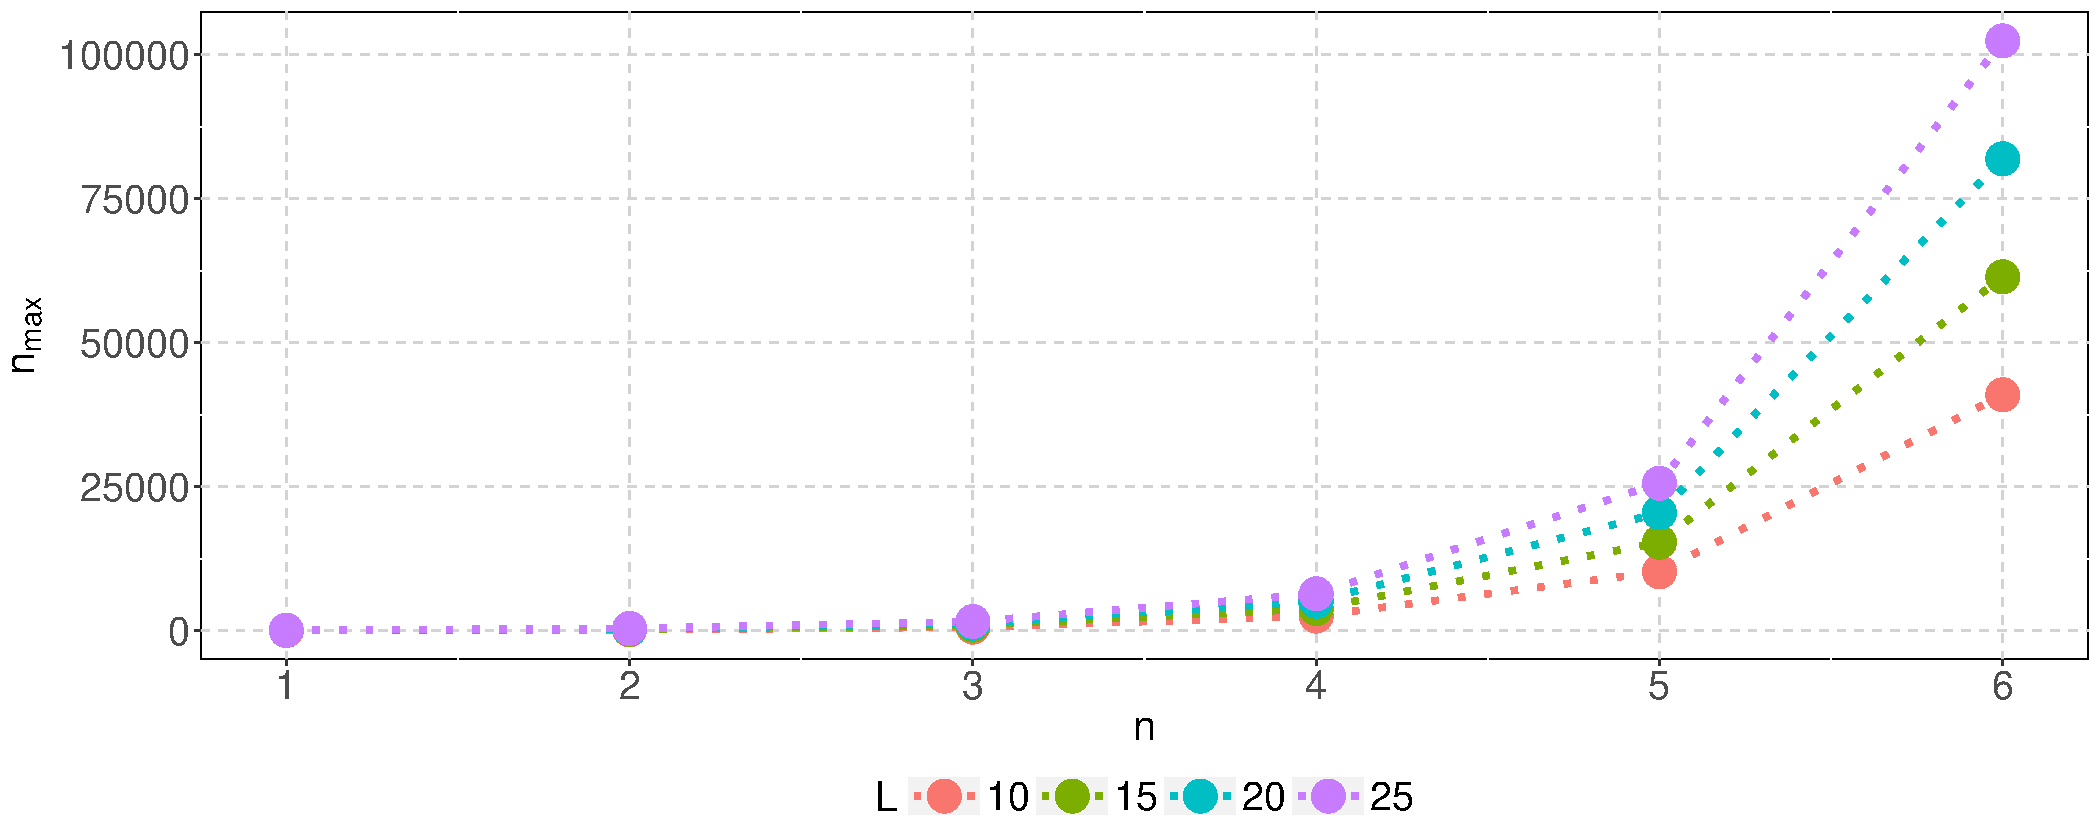
\includegraphics[width=\maxwidth]{figure/unnamed-chunk-4-1} 

}



\end{knitrout}

To decrease $m$, one may reduce the amino acid alphabet using heuristics provided in \textit{biogram}.

Function: \textit{reduce\_alphabet()}.


    \end{block}
    \vfill
    
    \begin{block}{Selection of important n-grams}
    Model and statistic independent permutation tests can be used to filter features obtained through counting n-grams.
    
    During a permutation test class labels are randomly exchanged during computation of a significance statistic. p-values are defined as:
    
\begin{center}
\scalebox{0.85}{
$      
\textnormal{p-value} = \frac{N_{T_P > T_R}}{N}
$
}
\end{center}

where $N_{T_P > T_R}$ is number of times when $T_P$ (permuted test statistic) 
was more extreme than $T_R$ (test statistic for non-permuted data).

Permutation tests are computationally expensive (especially considering precise 
estimation of small p-values, because the number of permutations is inversely 
proportional to the interval between p-values).

\bigskip

\textbf{Qui}ck \textbf{P}ermutation \textbf{T}est (QuiPT) thanks to the unique 
parameterization replaces a permutation test with the exact two-sided Fisher's 
test reducing the computation cost and returning more precise p-values. 
  

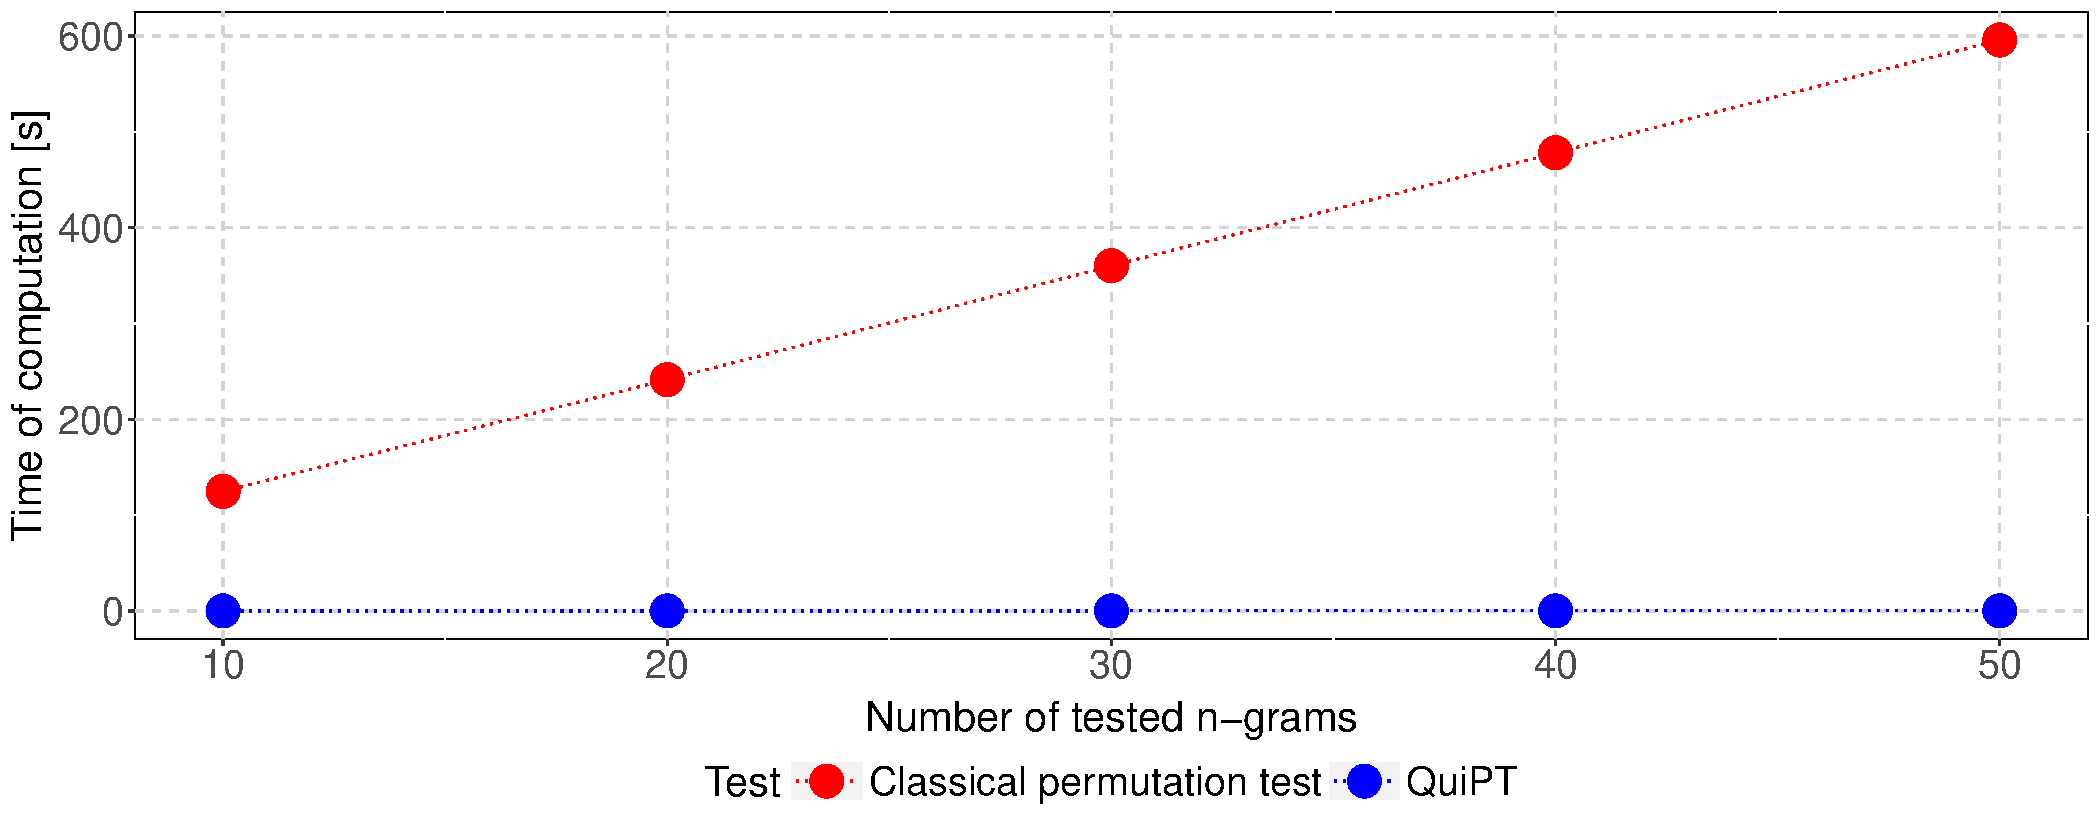
\includegraphics[width=\maxwidth]{figure/unnamed-chunk-5-1} 


Function: \textit{test\_features()}.

    \end{block}
    \vfill


    \begin{block}{Bibliography}
    \tiny{
      \bibliographystyle{apalike}
      \bibliography{signalhsmm_poster}
    }
    \end{block}
    \vfill 

}
\end{minipage}
\end{beamercolorbox}
\end{column}


%new column ------------------------------------------------------    

\begin{column}{.50\textwidth}
\begin{beamercolorbox}[center,wd=\textwidth]{postercolumn}
\begin{minipage}[T]{.95\textwidth}  
\parbox[t][\columnheight]{\textwidth}
{

\begin{block}{Case study: signal peptide prediction}

The computational methods for the recognition of signal peptides, 
short peptides tagging secretory proteins, accurately identify typical peptides, 
well-represented in protein databases~\citep{petersen_signalp_2011}. However, 
these algorithms are not general enough to predict signal peptides with unique 
amino acid composition, for example those present in proteins from malaria 
parasites. 
\end{block}

     \begin{block}{PCA of signal peptides and mature proteins}

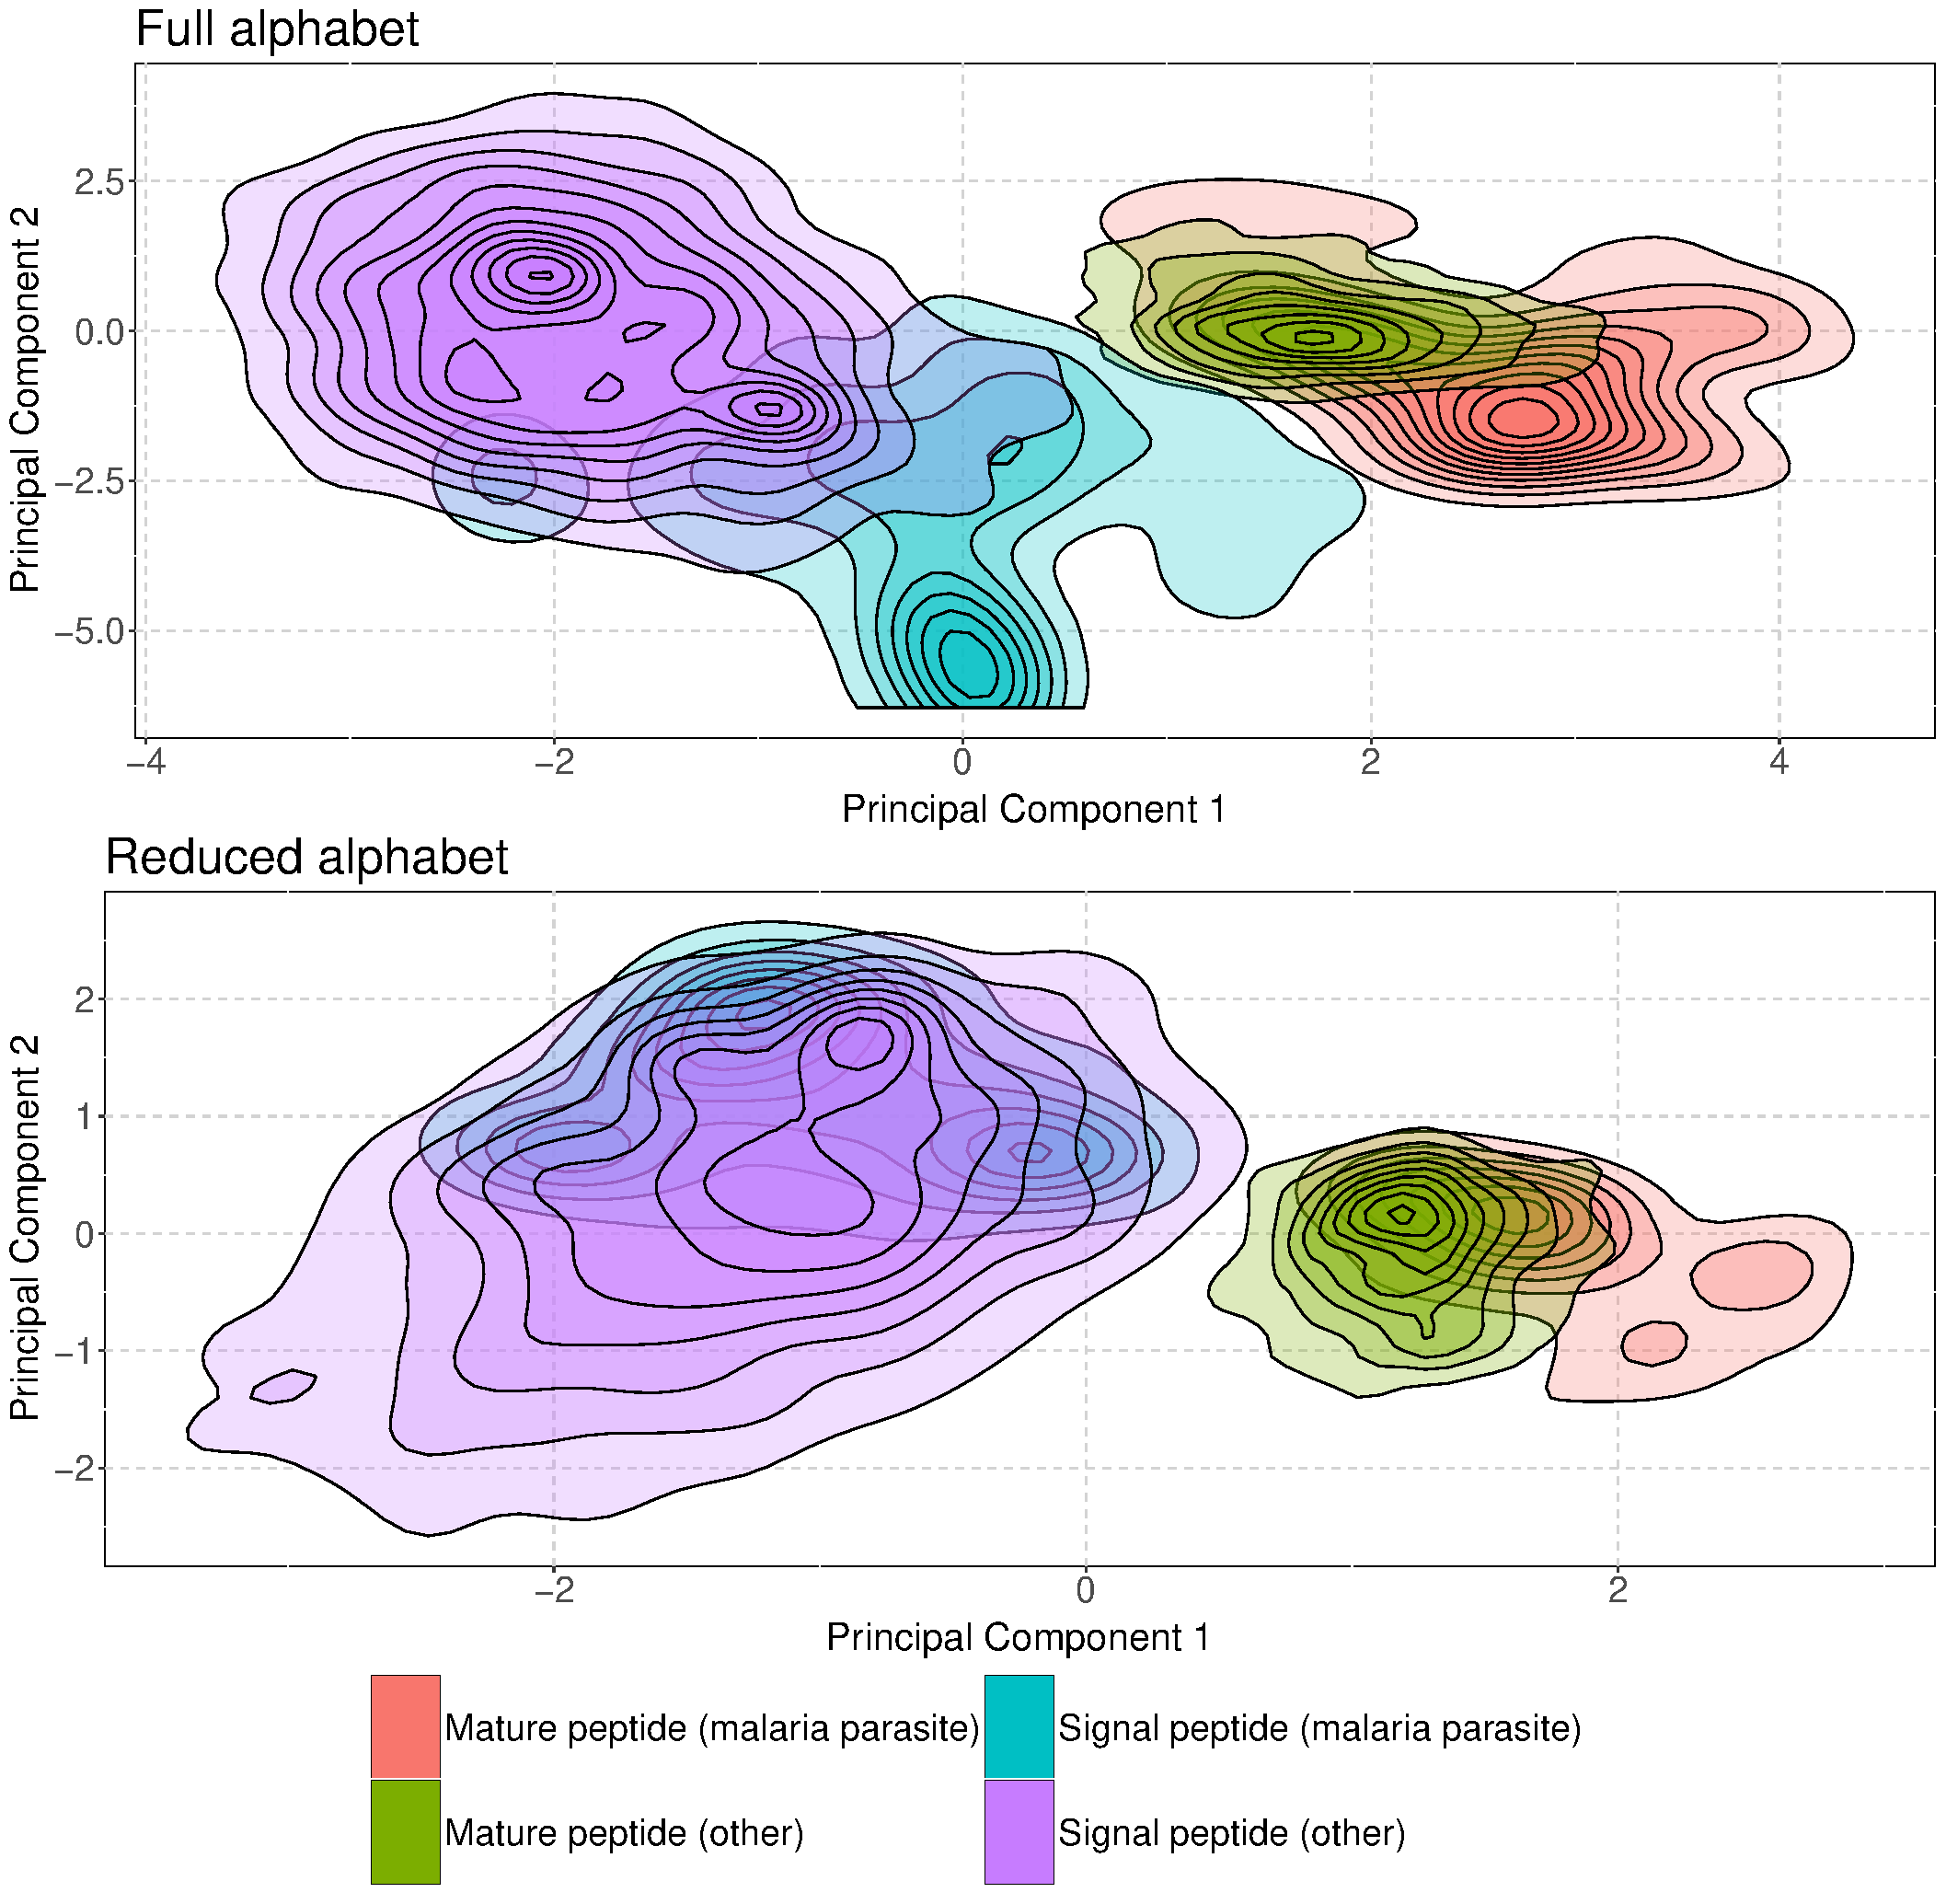
\includegraphics[width=\maxwidth]{figure/unnamed-chunk-6-1} 


A countour plot of first two components in Principal Component 
Analysis of amino acid frequency. The signal peptides from malaria and other 
taxons differ significantly when the full amino acid alphabet is employed. After 
the reduction of the alphabet, the signal peptides group together despite their 
origin.

\bigskip

Here, the reduction of the amino acid alphabet not only creates more manageable 
feature space, but also mimics the biology behind the process of the signal 
peptide recognition. Grouping of amino acids reflects their physicochemical 
properties which are important in protein secretion.

    \end{block}
    \vfill

    
    \begin{block}{Benchmark with other predictors of signal peptides}
    Benchmark data set: 51 proteins with signal peptide and 211 proteins 
    without signal peptide from malaria parasites.
    
    signalHsmm - n-gram based software for prediction of signal peptides.
   
    \begin{table}[ht]
\centering
\begin{tabular}{rllll}
  \toprule
 & Sensitivity & Specificity & MCC & AUC \\ 
  \midrule
signalP 4.1 \citep{petersen_signalp_2011} & 0.8235 & 0.9100 & 0.6872 & 0.8667 \\ 
   \rowcolor{white}signalP 4.1 (tm) \citep{petersen_signalp_2011} & 0.6471 & 0.9431 & 0.6196 & 0.7951 \\ 
   PrediSi \citep{hiller_predisi:_2004} & 0.3333 & \textbf{0.9573} & 0.3849 & 0.6453 \\ 
   \rowcolor{white}Philius \citep{reynolds_transmembrane_2008} & 0.6078 & 0.9336 & 0.5684 & 0.7707 \\ 
  Phobius \citep{kall_combined_2004} & 0.6471 & 0.9289 & 0.5895 & 0.7880 \\ 
   \rowcolor{white}signalHsmm & 0.9804 & 0.8720 & 0.7409 & 0.9262 \\ 
  signalHsmm (hom. 50\%) & \textbf{1.0000} & 0.8768 & \textbf{0.7621} & \textbf{0.9384} \\ 
   \rowcolor{white}signalHsmm (raw aa) & 0.8431 & 0.9005 & 0.6853 & 0.8718 \\ 
   \bottomrule
\end{tabular}
\end{table}
    \end{block}
    \vfill
     
    \begin{block}{Conclusions and funding}
    
    
    \texit{biogram} is a versatile toolkit for n-gram analysis of biological sequences in \textbf{R}.
    
    \bigskip
    
      Thanks to the reduction of amino acid alphabet, signalHsmm is able 
      to recognize signal peptides from the malaria parasites and their 
relatives more accurately than other software. 

\bigskip

\textit{biogram} repository: \url{https://github.com/michbur/biogram}

\bigskip

signalHsmm web-server: \url{http://www.smorfland.uni.wroc.pl/shiny/signalHsmm/}. 

\bigskip

Find us online: \url{https://github.com/michbur/USER2017}.      

\small{This research was partially funded by the KNOW Consortium and National Science Center (2015/17/N/NZ2/01845).}

    \end{block}
    \vfill 
    
        
     
    


}
\end{minipage}
\end{beamercolorbox}
\end{column}
\end{columns}  
\end{frame}
\end{document}
